\section{Model Description}
\subsection{Plackett-Luce observation model}
\textbf{Model 1} (without seniority covariates): We use a Plackett-Luce observation model for these data. In a Plackett-Luce model without covariates, each player $i=1, \ldots, n$ has a skill $\lambda_{i} \in R$. For $1 \leq m \leq n$ let $\left\{i_{1}, \ldots, i_{m}\right\}$ be a subset of $\{1,2, \ldots, n\}$ and let $\mathcal{P}_{i_{1}, \ldots, i_{m}}$ denote the set of all permutations of the labels $\left\{i_{1}, \ldots, i_{m}\right\}$. In a game with $m$ players with player labels $i_{1}, \ldots, i_{m}$, the outcome $O \in \mathcal{P}_ {i_{1}, \ldots, i_{m}}$ is a random permutation $o= \left(o_{1}, \ldots, o_{m}\right), o \in \mathcal{P}_{i_{1}, \ldots, i_{m}}$ of the player labels. In the Plackett-Luce model with $\lambda=\left(\lambda_{1}, \ldots, \lambda_{n} \right)$, the probability for the random rank-outcome $O$ of a single generic competition to be some particular ranking $o$ is
\begin{equation*}
\operatorname{Pr}\{O=o \mid \lambda\}=\prod_{i=1}^{m} \frac{\exp \left(\lambda_{o_{i}}\right)}{\sum_{j=i}^{m} \exp \left(\lambda_{o_{j}}\right)}
\end{equation*}

\textbf{Model 2} (with seniority covariates): A vector of seniority parameters $\beta=\left(\beta_{1}, \ldots, \beta_{n}\right)$ may be introduced so that the effect of having seniority-level $k, k=1, \ldots, n$ is $\beta_{k} \in R$. In this observation model
\begin{equation*}
\operatorname{Pr}\{O=o \mid \lambda, \beta\}=\prod_{i=1}^{m} \frac{\exp \left(\lambda_{o_{i}}+\beta_{e_{i}}\right)}{\sum_{j=i}^{m} \exp \left(\lambda_{o_{j}}+\beta_{e_{j}}\right)}
\end{equation*}
where for $i \in\left\{i_{1}, \ldots, i_{m}\right\}$ the index $e_{i}$ on $\beta_{e_{i}}$ gives the seniority rank of player $i$ at the time the game was played.

\subsection{Prior elicitation and checking}
In eliciting the priors for the skills $\lambda$ and the effects of seniority $\beta$ for each player, we should bare in mind that these priors should be non-informative with respect to the relative skills of the players and the advantage for seniority. In addition, the probability of all games outcomes corresponding to the set of all permutations of the labels $\left\{i_{1}, \ldots, i_{m}\right\}$ should be the same for any given subset $\left\{i_{1}, \ldots, i_{m}\right\}$ of $\{1,2, \ldots, n\}$. The domains of the parameters $\lambda \in R^{m}$, therefore, the class of $t$ distributions offers a good choice. We simulate $10,000$ samples from the priors $\lambda_{o_{i}} \stackrel{\text{i.i.d}}{\sim} t_5$ and plot the likelihood $\operatorname{Pr}\{O=o \mid \lambda\}$ for each random permutation $o \in \mathcal{P}_{1, 2, 3}$ of three players $\{1, 2, 3\}$ in Figure~\ref{fig:3a}. The densities of the likelihood function of the $3!$ outcomes match well. Marginalizing over $\lambda$, the estimate for the expectation $E_{\lambda \mid model} \left[ \operatorname{Pr}\{O=o \mid \lambda\} \right]$ of each permutation is close to $1/3!$, agreeing with our prior beliefs that all permutations $o \in \mathcal{P}_{1, 2, 3}$ are equally probable. The distribution becomes tighter as we use a lower degree of freedom $t_{1}$ (Figure~\ref{fig:3b}). The larger degree of freedom $t_{5}$ is desired as we want to be less certain about the likelihood of the outcomes due to the randomness of the game.
\begin{figure}[ht!]
\centering
\begin{subfigure}[b]{0.45\textwidth}
   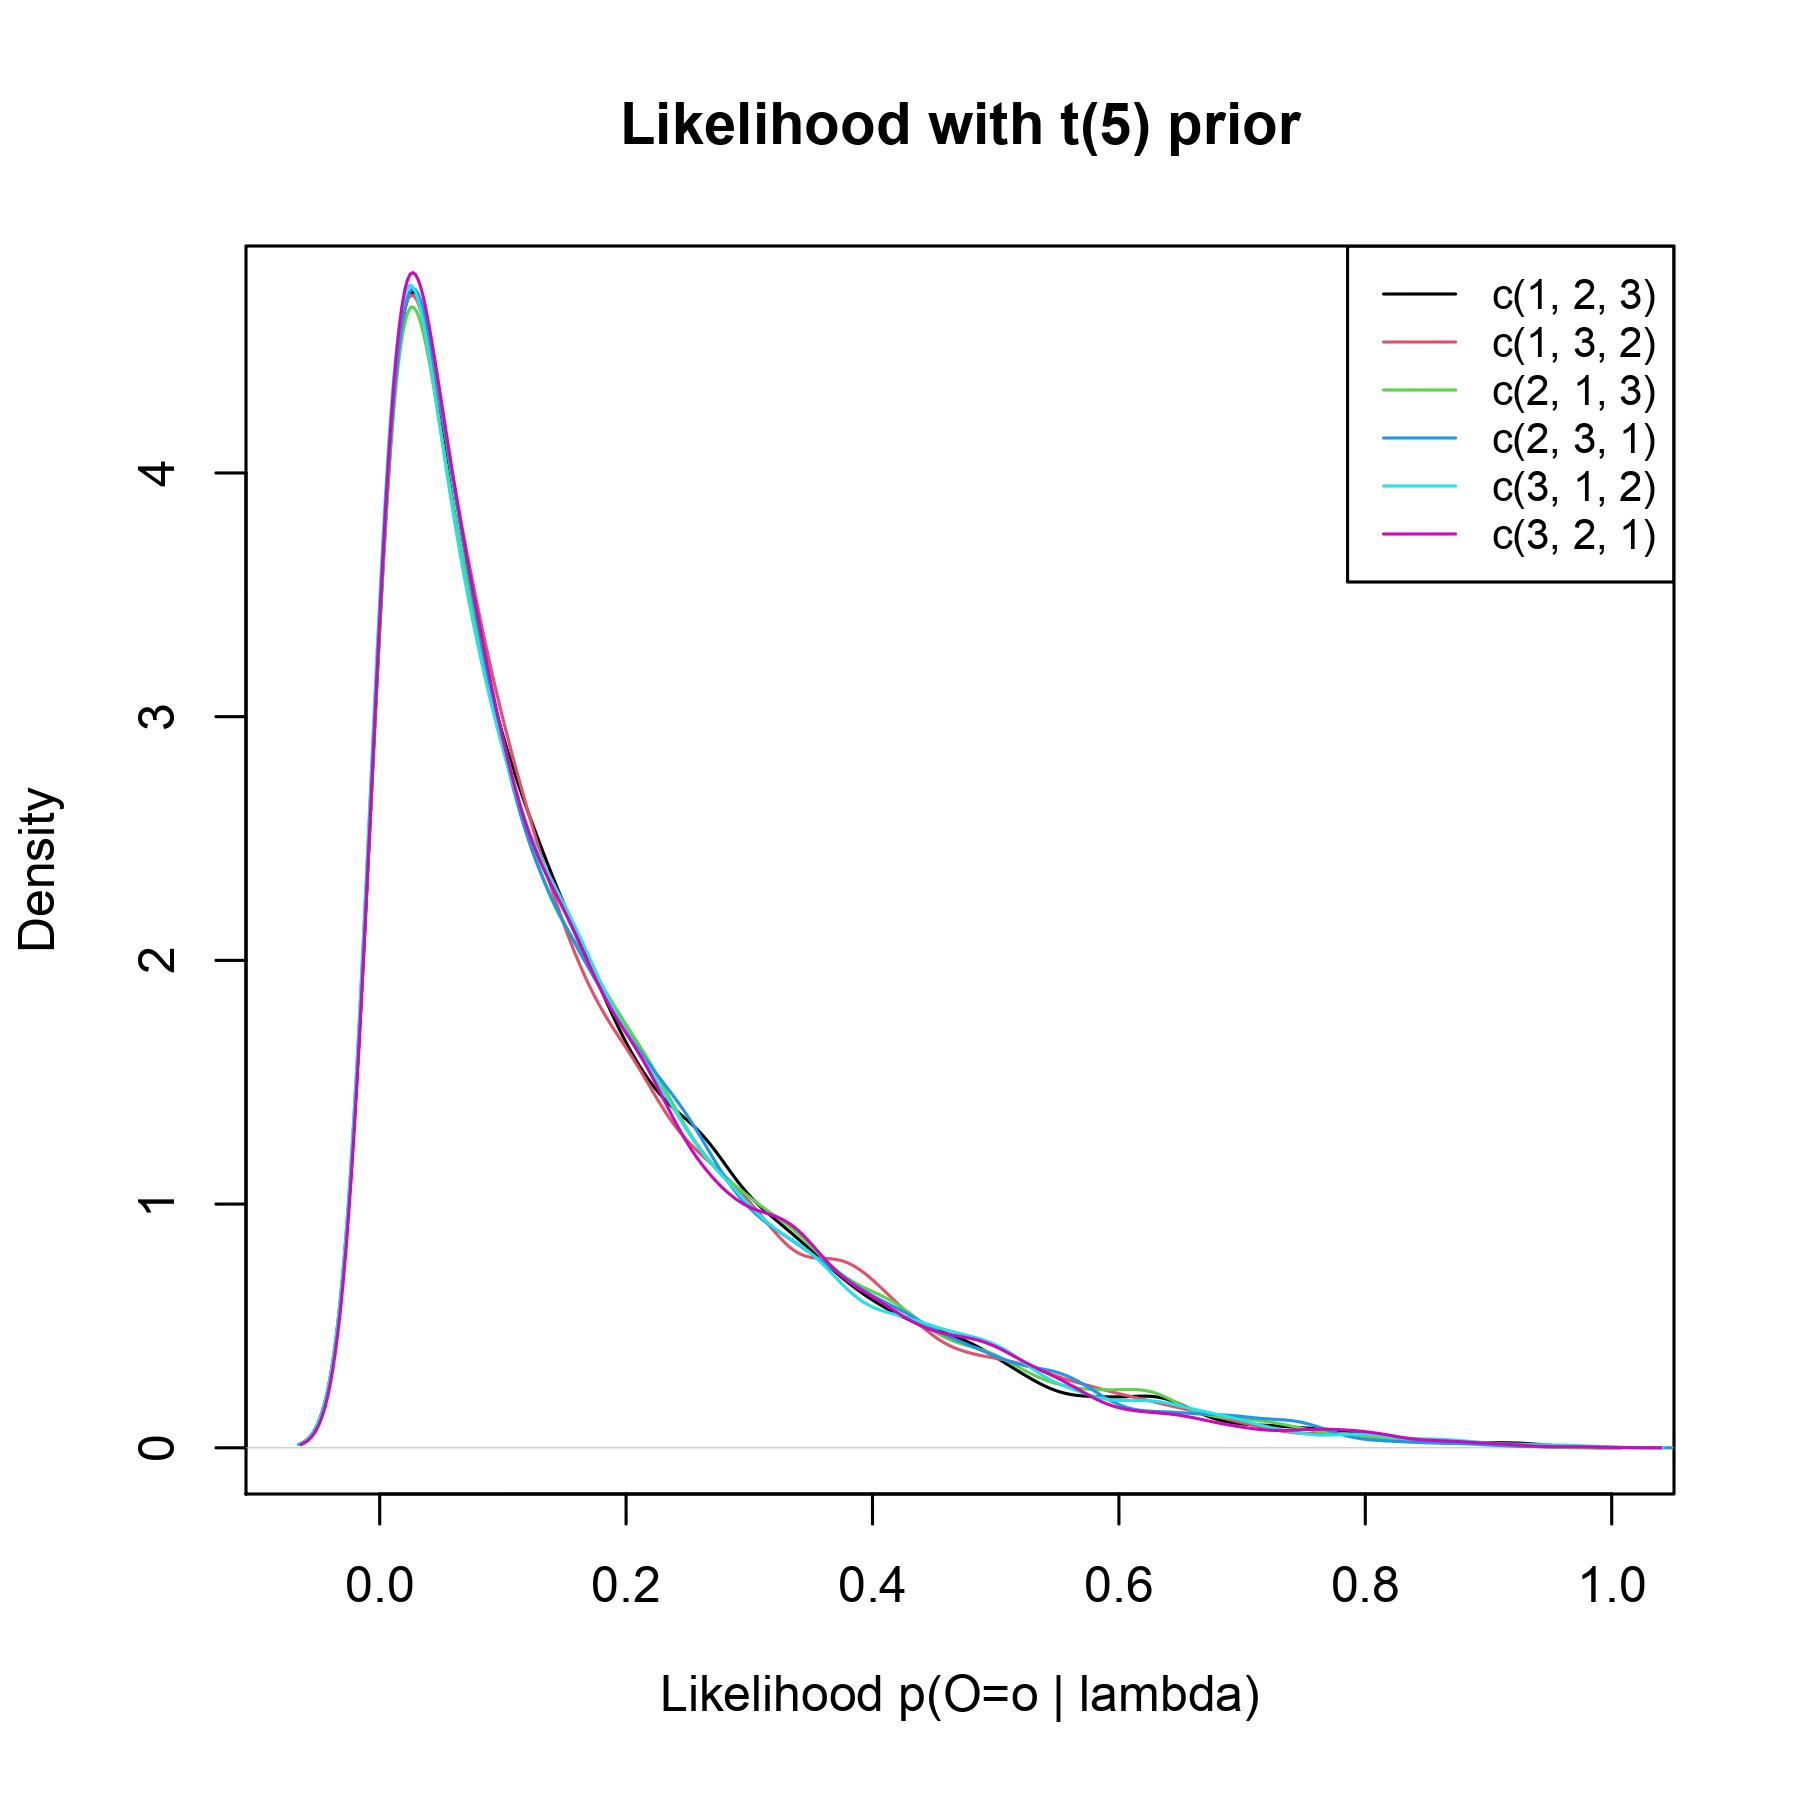
\includegraphics[width=1\linewidth]{one_t5}
   \caption{Model 1 likelihood with $t_{5}$ prior} \label{fig:3a}
\end{subfigure}
\begin{subfigure}[b]{0.45\textwidth}
   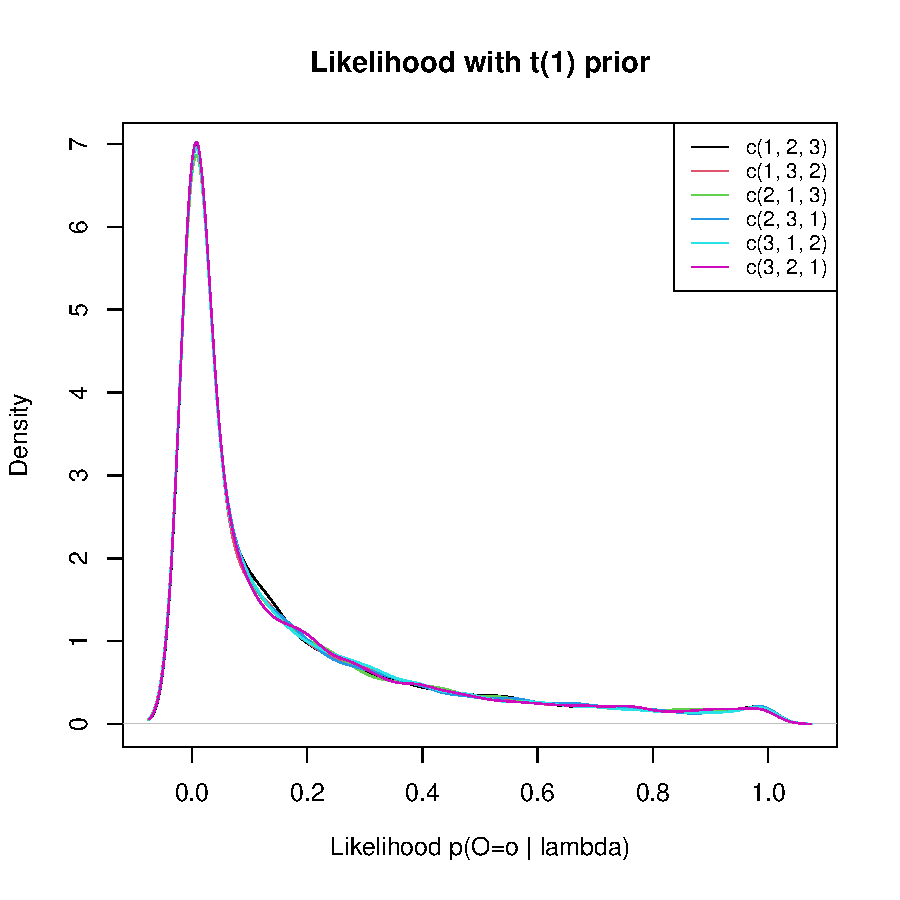
\includegraphics[width=1\linewidth]{one_t1}
   \caption{Model 2 likelihood with $t_{1}$ prior} \label{fig:3b}
\end{subfigure} \hspace{1em}
\caption{Likelihood densities of all $3!$ permutations of the labels $o \in \mathcal{P}_{1, 2, 3}$ in model 1 (with parameter $\lambda$). The densities of all outcomes match well, indicating the prior is non-informative with respect to the rankings of the players involved in the competition. The $t_{5}$ distribution with the larger degree of freedom gives less certainty about the outcomes and is desired.} \label{fig:3}
\end{figure}

We perform a similar check for model 2 with seniority covariates added, we choose the additional priors $\beta_{e_{i}} \stackrel{ \text{i.i.d}}{\sim} t_5$ and observe that the likelihood densities of all outcomes match. Again, a $t$ distribution with a larger degree of freedom gives less certainty about the outcomes. The estimate for the marginal likelihood $E_{\lambda, \beta \mid model} \left[ \operatorname{Pr}\{O=o \mid \lambda, \beta\} \right]$ is close to $1/m!$, matching our prior beliefs.
